% Created 2019-03-28 Thu 21:18
% Intended LaTeX compiler: pdflatex
\documentclass[10pt, compress, aspectratio=169, xcolor={table,usenames,dvipsnames}]{beamer}

\usepackage{booktabs}
\mode<beamer>{\usetheme[numbering=fraction, progressbar=none, titleformat=smallcaps, sectionpage=none]{metropolis}}
\usepackage{sourcecodepro}
\usepackage{booktabs}
\usepackage{array}
\usepackage{listings}
\usepackage{graphicx}
\usepackage[english]{babel}
\usepackage[scale=2]{ccicons}
\usepackage{url}
\usepackage{relsize}
\usepackage{amsmath}
\usepackage{bm}
\usepackage{wasysym}
\usepackage{ragged2e}
\usepackage{textcomp}
\usepackage{pgfplots}
\usepgfplotslibrary{dateplot}
\definecolor{Base}{HTML}{191F26}
\definecolor{Accent}{HTML}{790700}
\setbeamercolor{alerted text}{fg=Accent}
\setbeamercolor{frametitle}{bg=Base}
\setbeamercolor{normal text}{bg=black!2,fg=Base}
\setsansfont[BoldFont={Source Sans Pro Semibold},Numbers={OldStyle}]{Source Sans Pro}
\lstdefinelanguage{Julia}%
{morekeywords={abstract,struct,break,case,catch,const,continue,do,else,elseif,%
end,export,false,for,function,immutable,mutable,using,import,importall,if,in,%
macro,module,quote,return,switch,true,try,catch,type,typealias,%
while,<:,+,-,::,/},%
sensitive=true,%
alsoother={$},%
morecomment=[l]\#,%
morecomment=[n]{\#=}{=\#},%
morestring=[s]{"}{"},%
morestring=[m]{'}{'},%
}[keywords,comments,strings]%
\lstset{ %
backgroundcolor={},
basicstyle=\ttfamily\scriptsize,
breakatwhitespace=true,
breaklines=true,
captionpos=n,
commentstyle=\color{Accent},
extendedchars=true,
frame=n,
keywordstyle=\color{Accent},
language=R,
rulecolor=\color{black},
showspaces=false,
showstringspaces=false,
showtabs=false,
stepnumber=2,
stringstyle=\color{gray},
tabsize=2,
}
\renewcommand*{\UrlFont}{\ttfamily\smaller\relax}
\graphicspath{{../../img/}}
\addtobeamertemplate{block begin}{}{\justifying}
\setbeamertemplate{itemize/enumerate body begin}{\normalsize}
\setbeamertemplate{itemize/enumerate subbody begin}{\normalsize}
\usetheme{default}
\author{\footnotesize Pedro Bruel \newline \scriptsize \emph{phrb@ime.usp.br}}
\date{\scriptsize \today}
\title{Autotuning: A Design of Experiments Approach}
\hypersetup{
 pdfauthor={\footnotesize Pedro Bruel \newline \scriptsize \emph{phrb@ime.usp.br}},
 pdftitle={Autotuning: A Design of Experiments Approach},
 pdfkeywords={},
 pdfsubject={},
 pdfcreator={Emacs 26.1 (Org mode 9.2.2)},
 pdflang={English}}
\begin{document}

\maketitle

\section{Autotuning}
\label{sec:orga281e8e}
\begin{frame}[label={sec:org83d7101}]{Autotuning: Optimizing Program Configurations}
\begin{columns}
\begin{column}{0.5\columnwidth}
\begin{block}{Architectures for High Performance Computing}
\begin{center}
\includegraphics[width=.9\linewidth]{../../../img/architectures.png}
\end{center}

How to write \alert{efficient code} for each of these?

\begin{block}{Autotuning}
\vspace{.2cm}

The process of \alert{automatically finding} a \alert{configuration} of a program that
optimizes an \alert{objective}
\end{block}
\end{block}
\end{column}

\begin{column}{0.5\columnwidth}
\begin{block}{Popular Approaches to Autotuning}
\begin{itemize}
\item Exhaustive
\item Meta-Heuristics
\item Machine Learning
\vspace{-.2cm}
\end{itemize}

\begin{block}{Our Approach}
\begin{itemize}
\item \alert{Design of Experiments} (\alert{DoE})
\end{itemize}
\end{block}
\end{block}
\end{column}
\end{columns}
\end{frame}

\section{Design of Experiments}
\label{sec:org786a0d0}
\begin{frame}[label={sec:org64759d6}]{Design of Experiments: An Example on Agriculture}
\begin{columns}
\begin{column}{0.55\columnwidth}
\begin{center}
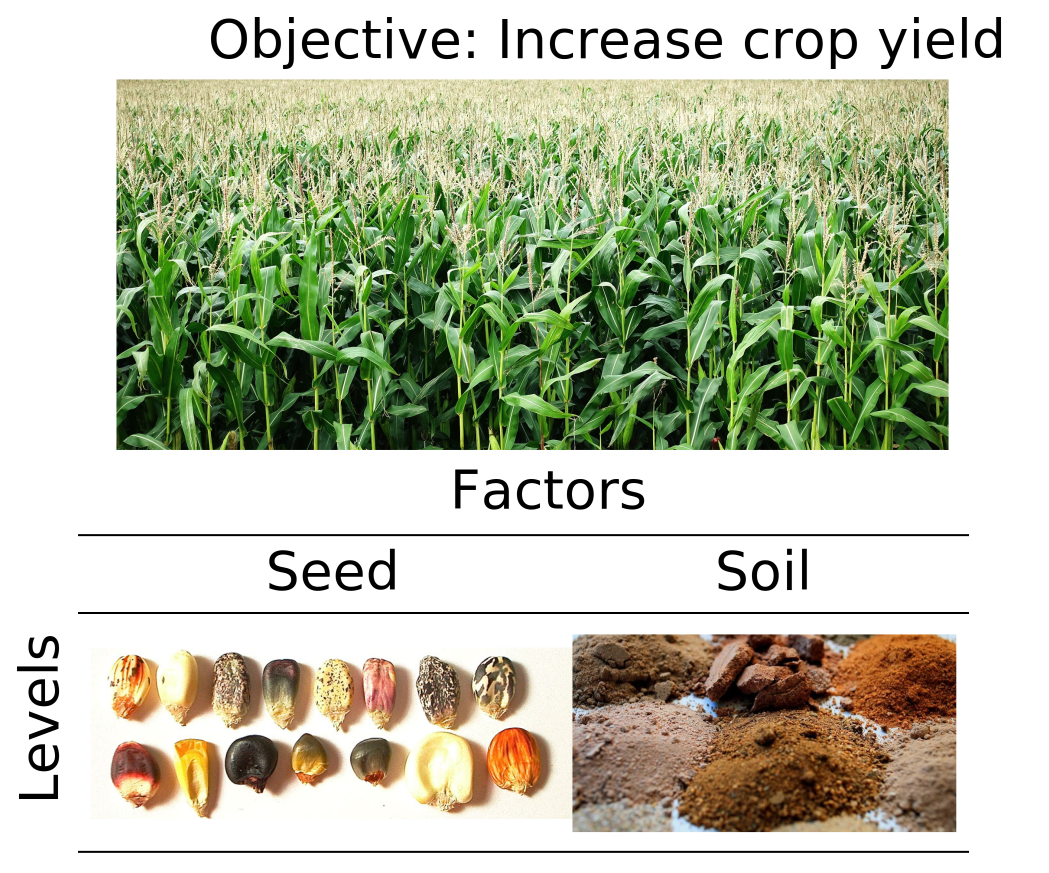
\includegraphics[width=.99\columnwidth]{../../../img/crop_yield_doe_example.pdf}
\end{center}
\end{column}
\begin{column}{0.45\columnwidth}
\begin{block}{Testing \alert{all combinations} is \alert{inviable}}
\begin{block}{Which combinations to test?}
\begin{itemize}
\item DoE provides a \alert{selection method}
\item \alert{Parsimony}: \alert{decreases experiments}
\end{itemize}
\end{block}

\begin{block}{Which is the best combination?}
\begin{itemize}
\item DoE provides an \alert{analysis method}
\item \alert{Transparency}: use \alert{statistical tests}
\end{itemize}
\end{block}

\begin{block}{\alert{How to use DoE on Autotuning?}}
\end{block}
\end{block}
\end{column}
\end{columns}
\end{frame}

\maketitle
\end{document}